\documentclass[conference]{IEEEtran}
\pdfoutput=1    % For arXiv issues


% -------------------------- COLORBLIND COLORS -------------------------------
% Use color palettes for colorblind people from
% https://davidmathlogic.com/colorblind/#%23D81B60-%231E88E5-%23FFC107-%23004D40 or https://colorbrewer2.org/
\usepackage{xcolor}
\definecolor{wong-black}        {HTML}{000000}
\definecolor{wong-lightorange}  {HTML}{E69F00}
\definecolor{wong-lightblue}    {HTML}{56B4E9}
\definecolor{wong-green}        {HTML}{009E73}
\definecolor{wong-yellow}       {HTML}{F0E442}
\definecolor{wong-darkblue}     {HTML}{0072B2}
\definecolor{wong-darkorange}   {HTML}{D55E00}
\definecolor{wong-pink}         {HTML}{CC79A7}

% -------------------------- PACKAGES -------------------------------

\usepackage{url}
\def\UrlBreaks{\do\/\do-}   % Line breaks of long URLs in biblatex bibliography (https://tex.stackexchange.com/questions/134191/line-breaks-of-long-urls-in-biblatex-bibliography)

\usepackage{hyperref} % Working hyperlink (https://www.overleaf.com/learn/latex/Hyperlinks)
\hypersetup{
    colorlinks=true,
    citecolor=wong-green,
    linkcolor=wong-darkblue,
    filecolor=wong-pink,      
    urlcolor=wong-black,
    pdfpagemode=FullScreen,
    }

% Use these to always use Fig. and Sec. instead of worrying about Figure, Fig, Fig. etc in the document
\newcommand{\figref}[1]{Fig.~\ref{#1}}
\newcommand{\secref}[1]{Sec.~\ref{#1}}

\usepackage{cite}
\usepackage{siunitx-v2}
\usepackage{tabularx}
\usepackage{booktabs}
\usepackage{amsmath,amssymb,amsfonts}
\usepackage{algorithmic}
\usepackage{multirow,graphicx}
\usepackage{textcomp}
\usepackage[nolist, nohyperlinks, printonlyused]{acronym} % For consistent acronyms
\usepackage{tablefootnote}
\usepackage{threeparttable}

\def\BibTeX{{\rm B\kern-.05em{\sc i\kern-.025em b}\kern-.08em
    T\kern-.1667em\lower.7ex\hbox{E}\kern-.125emX}}

%% orcid logo
\usepackage{scalerel}
\usepackage{tikz}
\usetikzlibrary{svg.path}


\definecolor{orcidlogocol}{HTML}{A6CE39}
\tikzset{
	orcidlogo/.pic={
		\fill[orcidlogocol] svg{M256,128c0,70.7-57.3,128-128,128C57.3,256,0,198.7,0,128C0,57.3,57.3,0,128,0C198.7,0,256,57.3,256,128z};
		\fill[white] svg{M86.3,186.2H70.9V79.1h15.4v48.4V186.2z}
		svg{M108.9,79.1h41.6c39.6,0,57,28.3,57,53.6c0,27.5-21.5,53.6-56.8,53.6h-41.8V79.1z M124.3,172.4h24.5c34.9,0,42.9-26.5,42.9-39.7c0-21.5-13.7-39.7-43.7-39.7h-23.7V172.4z}
		svg{M88.7,56.8c0,5.5-4.5,10.1-10.1,10.1c-5.6,0-10.1-4.6-10.1-10.1c0-5.6,4.5-10.1,10.1-10.1C84.2,46.7,88.7,51.3,88.7,56.8z};
	}
}

\newcommand\orcidicon[1]{\href{https://orcid.org/#1}{\mbox{\scalerel*{
				
\begin{tikzpicture}[yscale=-1,transform shape]
					\pic{orcidlogo};
				\end{tikzpicture}
			}{|}}}}
    
\newcommand\nnfootnote[1]{  % Footnote without hyperref association (https://tex.stackexchange.com/questions/415625/avoiding-hyperref-warning-ignoring-empty-anchor)
  \begin{NoHyper}
  \renewcommand\thefootnote{}\footnote{#1}%
  \addtocounter{footnote}{-1}%
  \end{NoHyper}
}

\begin{document}

% -------------------------- TITLE -------------------------------

\title{Definition of Test Oracles for Identifying TP, FP, and FN in Object Perception for Automated Driving}

%\title{Relevant Criteria for Identifying TP, FP, and FN in Dependability Assessment of Object Perception}


%\title{A Language to Specify a Test Oracle that Identifies TP, FP, and FN}


%\title{A Model to Define TP, FP, and FN for Dependable Object Perception}

% \title{A Model to Define True Positives, False Positives, and False Negatives for Dependable Object Perception}

% -------------------------- AUTHORS -------------------------------

\author{\IEEEauthorblockN{
		Michael Hoss$^{1} \orcidicon{0000-0001-9924-7596}$
	}

% \IEEEauthorblockA{\IEEEauthorrefmark{2}}
% \IEEEauthorblockA{\IEEEauthorrefmark{3}}
}

\maketitle

\nnfootnote{$^{1}$~The author is with RWTH Aachen University, Germany. {\tt\small \href{mailto:michael.hoss@rwth-aachen.de}{michael.hoss@rwth-aachen.de}}. 
\newline
Despite being the only author, the first person plural (``we") is used to comply with a common style of scientific writing. 
}

%\nnfootnote{\textasteriskcentered~These authors contributed equally}

% -------------------------- ACRONYMS -------------------------------

\begin{acronym}
    \acro{ml}[ML]{Machine Learning}
	\acro{cnn}[CNN]{Convolutional Neural Network}
	\acro{dl}[DL]{Deep Learning}
	\acro{ad}[AD]{Autonomous Driving}
\end{acronym}

% -------------------------- ABSTRACT -------------------------------


\begin{abstract}
%%Single paragraph up to 250 words. Mini-version of the paper that includes context, state of the art, why it is not good enough, the research question, the methods, the evaluation and conclusions.
Contemporary test methods for the perception subsystem of automated vehicles require a characterization of true-positive, false-positive, and false-negative object tracks. % general term for TP, FP, FN
The literature defines these concepts in various different ways, which impedes comparability across different works. 
To overcome this issue, this paper provides an exhaustive model to define these concepts as formally as possible.
The model generally describes the criteria for association of tracks under test to reference tracks. 
Emphasized details are object distance functions in state space including penalties and thresholds, multi-object association algorithms, reference data and labeling characteristics, geometric issues like fields of view and semantic areas, temporal issues like incomplete tracks, and generalizations to probabilistic world models and asynchronous time stamps. 
While a majority of aspects can be formalized, a case study illustrates the remaining challenges towards an entirely formal description. 





% Yannick feedback:
% - be more precise, more clear, and more confident in abstract
% - probably use a more standardized templated abstract strcture
% - maybe even put in abstract that I want to bring together the perception community and the v&v community


%Single paragraph up to 250 words. Mini-version of the paper that includes context, state of the art, why it is not good enough, the research question, the methods, the evaluation and conclusions.
Test methods for the perception subsystem of driving automation systems commonly identify true-positive (TP), false-positive (FP), and false-negative (FN) objects. % general term for TP, FP, FN
Despite a common understanding, the implementation of these concepts varies across testing activities.
However, clear definitions are needed for their comparability and for a potential usage within a safety case. 
Therefore, this paper provides a set of relevant criteria for identifying TP, FP, and FN objects. % in an ideally unambiguous way.
% The criteria generally cover 
%that cover the generation of reference objects and their association to objects under test. 
Emphasized details are the tested object representations (e.g. detections or tracks), reference sensor characteristics, labeling policies, object distance functions, % in state space including penalties and thresholds, 
multi-object association, fields of view, areas of importance, incomplete tracks, asynchronous time stamps, and probabilistic object representations. 
% While a majority of aspects can be formalized, a case study illustrates the remaining challenges towards an entirely formal description. 
We find it challenging to characterize all aspects relevant for identifying TP, FP, and FN through adequate formal criteria due to both the open context problem and the symbol grounding problem.
Nevertheless, we encourage practitioners to define these aspects in their publications as formally as feasible. 
Uncertainties in these definitions likely remain and should therefore be accounted for in the induction of safety claims from statistics of TP, FP, and FN. 

\end{abstract}

% -------------------------- KEYWORDS -------------------------------

% \begin{IEEEkeywords}
% testing, environment perception, automated vehicles
% % component, formatting, style, styling, insert
% \end{IEEEkeywords}

% -------------------------- CONTENT -------------------------------


\section{Introduction}
\label{sec:introduction}

\subsection{Motivation}

The task of object-based environment perception for automated driving systems (ADS) receives much focus through public perception challenges, % that benchmark different approaches.
which publish datasets of raw sensor data along with reference labels for training purposes. 
Their leaderboards then rank individual submissions according to their similarity to the non-public reference labels on the test part of the dataset.

Common metrics of such leaderboards consist of aggregations of true-positive objects (TPs), false-positive objects (FPs), and false-negative objects (FNs). 
These direct metrics from the perception domain are comprehensible, straightforward to compute, and highly popular, but not necessarily adapted to the driving task. 
For example, it is typically unclear which FPs or FNs also lead to vehicle-level failures. 
% Assuming that every FP and FN leads to a vehicle-level failure would render the achievement of 
%Assuming that every FP or FN leads to a vehicle-level failure would be a tremendous overestimation that would 

To reduce and forecast vehicle-level failures, the field of safety assurance for automated driving has gained much popularity. 
One method of achieving provable safety is to decompose the driving automation system into different subsystems and establish dependable interfaces between them. 
The perception subsystem can be defined to consist of sensor hardware and computation for world modeling, excluding any prediction or planning into the future. 
Its dependability requires a sufficiently low mean time between events that induce vehicle-level failures. 
%Demonstrating this dependability is an active research questions that this paper aims to contribute to. 

% Or at least estimate how the perception outputs differ from the ground truth to construct sensor models for simulation tests.

The demonstration of this dependability is an active topic of research, where one of the most crucial issues is the identification of perception outputs that are not safe for the driving task. 
Task-oriented and safety-relevant perception metrics are therefore currently being proposed. 
In contrast to the most popular perception leaderboard metrics, safety-oriented metrics tend to be more complex and incomprehensible due to their additional consideration of the downstream driving function and of safety in road traffic. 
%Popularity of direct metrics that are based on TP, FP, FN still orders of magnitude higher than the popularity of task-oriented metrics. 

Ideally, novel perception metrics combine all desired properties such that they are helpful to both perception developers and verification and validation engineers. 
This requires closing the gap between straightforward safety-agnostic metrics and highly complex safety-relevant metrics. 
%comprehensible to humans, and straightforward to compute all at the same time. 

\subsection{Contributions}
\label{sec:introduction_contrib}
While one could make safety-relevant metrics less complex, the present paper aims at making straightforward metrics better usable for safety assurance. 
Specifically, we aim at defining TPs, FPs, and FNs clearly enough such that statistics of them represent meaningful evidences for safety claims \cite{Borg2022smirk}. 
%Differentiation between metric types:
%In contrast, downstream metrics from the safety domain are adapted to the driving task, but more difficult to understand, more difficult to compute, and still not as well researched. 
%These metrics, however, directly detect and penalize failures relevant to the driving task. 
%Consequently, we consider it worth while investigating whether metrics can be both easy to compute \textit{and} sufficient for safety claims.
%Context of this contribution:
%This paper provides potential tools for the definition of further perception metrics that are ideally task-oriented, safety-oriented, and easy to understand and compute. 
%Specifically, we aim at defining popular aspects of direct metrics clearly enough such that they can represent meaningful evidences for safety-relevant claims.  
Our main contributions are:
\begin{itemize}
\item A set of criteria to define how a test oracle identifies TPs, FPs, and FNs (Sec. \ref{sec:criteria})
\item A discussion of the relevance of TPs, FPs, and FNs in the safety assurance context (Sec. \ref{sec:discussion})
\end{itemize}


%This paper aims at contributing basic understanding of relevant at the intersection of perception and safety assurance. 


%Within the challenge to define useful safety-relevant perception metrics, this paper aims at 

%Can popular metrics based on TP, FP, and FN be adapted towards meaningful contributions within a safety case? 




The discussion will treat the following research questions:
\begin{itemize}


\item {RQ1}: \textit{Can TP, FP, and FN be objectively defined?}

\item {RQ2}: \textit{How relevant are TP, FP, and FN for task-oriented perception metrics?}

\item {RQ3}: \textit{Can statistics of TP, FP, and FN contribute to a safety argumentation?}
\end{itemize}

\begin{figure*}[t]
	\centering
	\vspace*{2mm}
	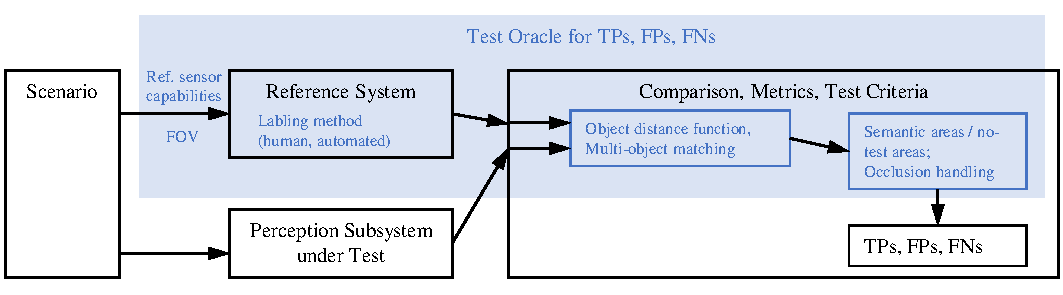
\includegraphics[width=\textwidth]{img/taxonomy_with_oracle.pdf}
	
	\caption{Test oracle for identifying TPs, FPs, and FNs, mapped into the taxonomy for ADS perception testing \cite{Hoss2022review, stellet2015testing}. Implemented test oracles can differ from this exemplary illustration. For example, certain aspects can be located either under ``Reference System" or ``Comparison, Metrics, Test Criteria".
		% TODO: insert subsection numbers.
	}
	\label{fig:oracle_in_taxonomy}
\end{figure*}


\subsection{Definition of terms \& abbreviations}
Unless stated otherwise, the following term definitions and acronyms hold throughout this paper.

\subsubsection{Object} \label{def:object}
From ISO 23150:2021 \cite{ISO_23150_2021_data_communication}: 
``representation of a real-world entity with defined boundaries and characteristics in the vehicle coordinate system".
This paper narrows down this definition to Layer 4 of the 6-layer-model \cite{Scholtes20216lmAccess}. An object can span over one or multiple time steps. 

\subsubsection{Object under Test (OuT)} \label{def:out} Perception subsystem of a driving automation system. It comprises both hardware and software and it outputs an object list in each time step. Note: The ``object" in OuT must not be confused with the more general \textit{object} defined above (Sec. \ref{def:object}).

\subsubsection{True Positive (TP)} \label{def:tp} The circumstance that an object in the data under test matches with an object in the reference data (Fig. \ref{fig:top_down_all}, 1).

\subsubsection{False Positive (FP)} \label{def:fp} The circumstance that an object in the data under test does not match with any object in the reference data (Fig. \ref{fig:top_down_all}, 2). 

\subsubsection{False Negative (FN)} \label{def:fn} The circumstance that no object in the data under test matches with a given object in the reference data (Fig. \ref{fig:top_down_all}, 3).

\subsubsection{True Negative (TN)} \label{def:tn} The circumstance that the non-existence of an object in the data under test matches with the non-existence of an object in the reference data. Since world modeling in form of object lists represents the non-existence of objects only implicitly, TNs are not quantifiable in the context of this paper.

%\subsubsection{Matching method} \label{def:matching_method} Those parts of the test method that influence the identification of TPs, FPs, and FNs. 
% based on an object list under test and a reference object list. 

% OMG I finally got the difference between method and methodology!! I should use method much more often now. But sometimes, methodology is the term to use (when I analyze different methods).

%\subsubsection{Matching result} \label{def:matching_result} General term or category of the mutually exclusive circumstances TP, FP, FN.  


%\subsubsection{Matching} As part of a test method, identifying TPs, FPs, and FNs based on the object lists of OuT and reference system. 

\subsubsection{Object association} \label{def:association} As part of a perception algorithm, deciding which existing object track a novel object detection belongs to. Not to be confused with \textit{matching}, which is a concept of the test method (adopted from \cite{Luiten2020hota}).

\subsubsection{(Test) oracle} \label{def:oracle} 
%The mechanism that determines whether a test passes or fails (see also survey by Barr et al. \cite{Barr2015oracle}).
In the present paper, \textit{(test) oracle} refers to the mechanism that identifies TPs, FPs, and FNs, where the test scenario and the OuT are given (Fig. \ref{fig:oracle_in_taxonomy}).

\subsubsection{Reference System (ReS)}
\label{def:reference_system}
Perception system that observes the scenario and whose outputted object list serves as a desired reference for the object list under test. 

% oracle problem in \cite{Zhang2022ml_testing}


\section{Methods}
\label{sec:method}

% We define the criteria for identifying TP, FP, and FN in the following way.

When human experts observe a top-down view representation of a traffic scene with an overlaid object list under test (Fig. \ref{fig:top_down_all}), they can typically make the following statements:
\begin{itemize}
	\item the ADS \textit{did} see the other road user
	\item the ADS \textit{did not} see the other road user 
	\item the ADS saw a road user \textit{that did not exist}.
\end{itemize}

We currently assume that an ideal test oracle exactly reproduces such human expert statements when it identifies TPs, FNs, and FPs correspondingly.
A human reference for the definition of a test oracle is beneficial for the human comprehensibility of the overall safety argumentation. 
However, for the sake of comparability of test results, the actual oracle should ideally be exactly reproducible and therefore contain as little human intuition as possible. 

Consequently, we aim at encoding our human intuition for a test oracle into unambiguous criteria. 
Our method to do this primarily consists of noting down and structuring all aspects that we consider relevant based on our previous experience. 
This experience consists of object-level online data fusion, object-level perception error modeling, testing of object perception against aerial reference data, and scenario elicitation from traffic recordings for safety assurance. 


As we apply this experience-based oracle definition to a popular perception challenge (Sec. \ref{sec:case_studies}), we refine it and demonstrate its practical applicability. 


%oracle is also at least partially based on intuition that is naturally impossible to specify explicitly. 
%Therefore, we intend to define criteria that allow to specify this human intuition as close as possible. 


%Eliminating the uncertainty of human intuition from the test oracle might make it more rigorous and formal, but for the time being, we justify our human reference for the test oracle as follows. 
%Since the safety argumentation is performed and evaluated by humans, its claims and evidences should be 


%\footnote{Eliminating informal human intuition from the oracle for TPs, FPs, and FNs could be beneficial, but this topic is outside the scope of this paper.}. 
%This assumption can be justified by the fact that human judges 


% Our goal is to list all relevant aspects of the test method 

%While other works use machine learning in the test method to reproduce these human observations \cite{Florbaeck2016.matching.offline, Sondell2018}, our goal is to make the features, criteria, and thresholds of the oracle as explicit as possible.



  



% Experience. No special method. 



\section{Definition of a test oracle for TPs, FPs, FNs}
\label{sec:criteria}



\begin{figure*}[t]
	\centering
	\vspace*{2mm}
	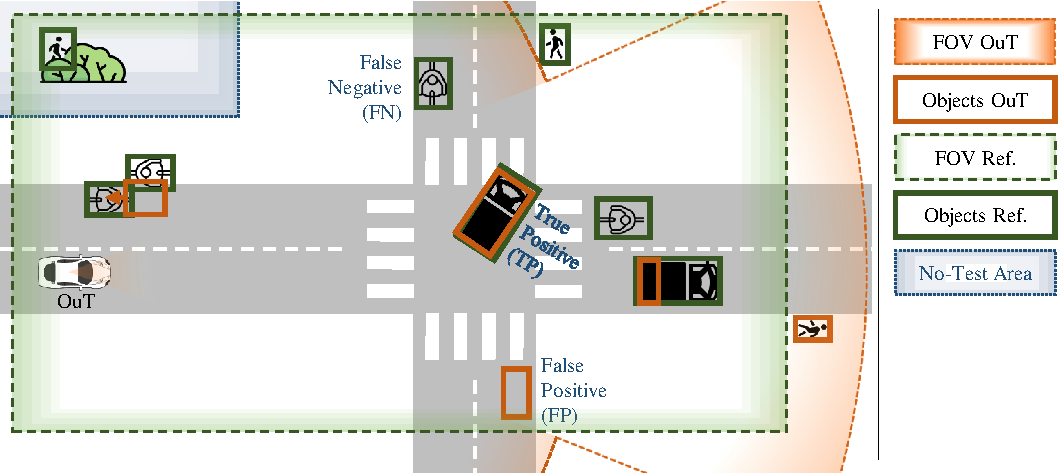
\includegraphics[width=\textwidth]{img/top_down_fitting_slide.pdf}
	
	\caption{ While objects A-C appear obvious, the desired identification of TPs, FPs, and FNs from objects D-L requires a purposefully defined test oracle. 
		%A clear definition of the test oracle is needed to understand how it identifies TPs, FPs, and FNs from the given objects A-L. 
		%Aspects of road traffic and geometry that the test oracle covers.
	}
	\label{fig:top_down_all}
\end{figure*}


A test oracle that identifies TPs, FPs, and FNs is a logical part of a testing activity (Fig. \ref{fig:oracle_in_taxonomy}), it deals with spatial relations in a traffic scene (Fig. \ref{fig:top_down_all}), and with temporal aspects of object matching (Fig. \ref{fig:timeline}).

This section details the aspects illustrated in the mentioned figures in natural language. 
% We intentionally avoid a more formal, more technical, or more specific description in order to keep it generally applicable to as many test oracles as possible without prescribing an internal structure and without . 
% DO THIS WHY NATURAL LANGUAGE HERE IN THE DISCUSSION!
It first treats the simple case of deterministic object representations in a single time frame (Sec. \ref{sec:oracle_simple}) and then covers temporal aspects (Sec. \ref{sec:oracle_time}) and probabilistic object descriptions (\ref{sec:oracle_probabilistic}).
The actual aspects that collectively define the workings of the test oracle are given one level of section structure deeper (e.g. Sec. \ref{sec:fov_ref}, \ref{sec:ref_hw}, \dots). 

%In this whole section, we assume that any FP or FN is an undesired penalty to the OuT. % is is just "one system saw something that the other system did not see" or is it "" MAYBE DEAL WITH THIS TOPIC IN ANOTHER SECTION??

%In general: matching of tracks under test to reference tracks. This boils down to:

\subsection{Matching deterministic objects in a single time frame}
\label{sec:oracle_simple}

In this subsection, we assume that the object lists of OuT and ReS are perfectly temporally synchronized. 

\subsubsection{Field of view of reference data}
\label{sec:fov_ref}
In general, the fields of view (FoV) can differ between OuT and ReS. This can lead to undesired FNs and FPs in areas where only one of both FoVs is present. 
In Fig. \ref{fig:top_down_all}, the OuT has no chance to detect pedestrian E, given its FoV. 
Likewise, the ReS has no chance to detect pedestrians K and J, given its FoV. 

Differing FoVs can have multiple reasons, such as different perspectives, different sensor choices, and different data processing methods, all of which are briefly explained in the following.
First, the perspective of a camera-equipped drone results in a rectangular FoV, whereas the OuT's FoV on the ground typically consists of circles and circular sectors (Fig.~\ref{fig:top_down_all}).
Second, reference data could be labeled only on the ego vehicle's cameras and lidars, whereas the OuT additionally uses a radar whose range exceeds the cameras and lidars used for the ReS. 
Third, even if OuT and ReS share the same sensors, in distant regions with sparse raw data, a manual labeling process of the ReS could reach either farther or shorter than the OuT's automated detection.
%their sensor ranges might not have clear-cut limits, but instead degrade probabilistically with increasing distance. In this probabilistic zone of performance degradation, the OuT's detection algorithm might propose object hypotheses where the ReS already refuses to label objects.

Whether or not the OuT should be penalized for missing pedestrian E in Fig. \ref{fig:top_down_all} depends on the test objective. 
If only the perception software is tested, then one might want to remove all objects from overhanging areas of the ReS to enable a fair evaluation.
However, if the sensor hardware's FoV of the OuT is put under test, too, and it is supposed to cover the entire ReS's FoV, then the ReS's FoV should not be trimmed and pedestrian E should be identified as a FN. 

In summary, a clear definition of the ReS's FoV relative to the OuT's FoV is crucial for a clearly defined test oracle. 

\subsubsection{Perspective-related occlusions}
\label{sec:occlusions}

If OuT and ReS observe the scenario from different perspectives, certain traffic participants can be visible for one system, but occluded for the other, which can lead to FPs and FNs. 
In Fig.~\ref{fig:top_down_all}, truck A occludes both cyclist G and pedestrian K for the OuT. 
Cyclist G, which is still within the ReS FoV, may be identified as a FN or be excluded from the evaluation due to the following reasons. 

On the one hand, the OuT could have tracked cyclist G through the temporary dynamic occlusion or it even could have perceived it by radar beams that go below truck A. 
On the other hand, one could argue that the OuT does not need to see behind any such occlusions if for safety reasons, the downstream behavior planning module assumes a road user behind such occlusions anyway.




\subsubsection{Reference system hardware}
\label{sec:ref_hw}

The way in which the ReS hardware differs from the OuT hardware influences the test oracle's identification of TPs, FPs, and FNs. 
In the simplest case, ReS and OuT share the very same sensor hardware and just differ in their data processing. 
This case would exclude unexpected FPs and FNs based on hardware differences, which is desired if only the OuT's software/data processing is focused. 

If, however, also the OuT's hardware is focused, then the ReS should be superior enough to identify the OuT's hardware limitations. 
For example, if the ReS hardware is better adapted to adverse weather conditions, it could detect objects that the OuT cannot detect (FNs) or confirm the real-world absence of ghost objects (FPs). 
%Depending on what part or parts of the OuT is focused in the testing activity (hardware/data processing), these FNs can be desired or undesired.




\subsubsection{Reference system labeling and data processing}
\label{sec:ref_processing}

The method by which an object list is extracted from the raw reference data influences the test oracle's identification of TPs, FPs, and FNs. 
This method can consist of programmed software, machine-learned modules, and human interaction. 

Labeling policy specifications, as being used by perception challenges and for outsourcing labeling activities to subcontractors, describe this extraction of object lists from raw reference data. 
These labeling policies include details such as how objects are classified, criteria for including and omitting objects, which parts of objects shall be inside or outside their bounding boxes, or how to label in case of partial or full occlusions\footnote{\url{https://github.com/waymo-research/waymo-open-dataset/blob/master/docs/labeling_specifications.md}}.

Even with a well-defined labeling policy, the actual labels can be uncertain \cite{wang2020inferring} or might sometimes differ from the policy. 
Therefore, test oracle is defined more clearly if the labeling is characterized also beyond its policy specification.
%For example, labeling can be fully automated, semi-automated, or manual, where each way impacts the labeling quality in a different way. 

On the one hand, this further characterization can include the internal workings, such as 
%This aspect of the test oracle can be characterized by its internal workings and its outputted results. 
the programmed modifications that the data undergo, the exact machine learning processes of any machine-learned modules, and the human interventions (when and how do humans manually label or otherwise interact with the data).
On the other hand, the ReS labeling and data processing can be further characterized by statistics about labeling accuracy and precision regarding state, classification, and existence of objects.
A higher-level reference system or evaluation procedure (``reference of the reference") would be needed for this purpose.


\subsubsection{Semantic areas and no-test areas}
\label{sec:semantic_areas}

Certain areas on or next to the road surface might be irrelevant to the traffic scenario and therefore be not worth while perceiving. 
To avoid needless test efforts, one could define no-test-areas, where no evaluation of TPs, FPs, and FNs takes place (Fig.~\ref{fig:top_down_all}, pedestrian D). 
For example, the KITTI object development kit\footnote{\url{https://www.cvlibs.net/datasets/kitti}} contains \textit{DontCare} labels where no reference data was labeled. 

The exclusion of objects from such areas can occur in different stages of the testing activity (Fig. \ref{fig:oracle_in_taxonomy}). 
They might already be excluded from the reference data; they might be included in the reference data, but excluded from the identification of TPs, FPs, and FNs; or, they could still be part of the TPs, FPs, and FNs, but excluded in a potential further evaluation.

In any case, a clear definition of no-test areas is crucial for a comprehensible test oracle. 
They could be defined by individual polygons or by generally applicable rules (e.g. farther away than \SI{20}{\meter} from any road surface or sidewalk).
The definition of no-test areas can be delicate due to the risk of omitting objects that are in fact safety-relevant. 
For example, pedestrian D in Fig.~\ref{fig:top_down_all} might be running towards the intersection or be throwing objects at it.

\subsubsection{Coordinate transformation from ReS to OuT}
\label{sec:geometrical_alignment}

Comparing the OuT's object list to the ReS object list requires both to be in the same coordinate system. 
Typically, the OuT's vehicle coordinate system is used for the comparison. 
Therefore, if the ReS internally uses a distinct coordinate system, the ReS object list must be transformed to the OuT's coordinate system. 

Ideally, uncertainties inherent in this geometric alignment are negligible. 
However, these uncertainties can skew the reference objects' positions, which affects the pairwise object distances for object matching (Sec. \ref{sec:distance_function}), which, in turn, affects the resulting TPs, FPs, and FNs.  
 
Especially, inaccuracies in the sensor orientation angles result in large cartesian offsets in a large radial distance from the sensor.
For reference sensors on the ego vehicle, such uncertainties could stem from the calibration of sensor mounting positions. 
For external reference sensors such as moving drones or mounted infrastructure sensors, the geometrical alignment has further challenges. %there are multiple ways of ending up with a common coordinate system.  
This includes a generally uncertain localization of the ego vehicle and of the external sensor because of uncertainties in RTK-GNSS measurements, uncertainties in localization on a map, uncertainties in determining position and orientation of the ego vehicle by the ReS, and the non-trivial transformation from the aerial perspective to a cartesian system over the ground. 

A comprehensively defined test oracle should therefore state the positional uncertainty resulting from the geometrical alignment to illustrate how this can affect the matching of object pairs.

\subsubsection{Object distance function for matching}
\label{sec:distance_function}

Once both object lists share the same coordinate system, the pairwise distances between ReS objects and OuT objects can be computed to find candidates for TPs. 
Commonly used distance functions are the euclidean distance between bounding box centroids, with common threshold values around \SI{2}{\metre}; or $1 - IoU$, where the threshold value could be $0.5$.
Some employed distance functions also qualify as mathematical metrics in a vector space of objects.

The chosen distance function and threshold values directly affect the identification of TPs. 
While the bounding boxes of truck A (Fig.~\ref{fig:top_down_all}) should match for any reasonable choice, the situation is less obvious for truck H.
Since only its rear end got detected by the OuT, both the centroid distance and $1 - IoU$ could prevent a match under the exemplary thresholds. 
Without a match, though, truck H would lead to a FP and a FN, which might be undesired given the fact that its property that is relevant to the driving task of ego vehicle, namely its rear end, got properly detected. 
Still, thresholds should also not be unnecessarily large to prevent unrelated misdetections such as G and B from merging into an undesired TP candidate.

%including penalties (object classifications?) and thresholds. 

Furthermore, an object pair that falls below the distance function's threshold does not automatically represent a TP. 
For example, the OuT bounding box of cyclist F (Fig.~\ref{fig:top_down_all}) could have a below-threshold centroid distance to both ReS bounding boxes nearby. 
If only a 1:1 matching is allowed (Sec. \ref{sec:multi_object_matching}), situation F would hold one TP and one additional FN.

If not only statistics, but also individual occurrences of FPs and FNs are important to the testing approach, one might have a preference about which ReS bounding box the OuT cyclist F should be matched with. 
For example, if the matched cyclists should go into the same direction, the distance function could include additional penalty terms for differing velocities or heading angles, which is already popular for distance functions in online object tracking. 

Additionally, the matching of vulnerable road users (VRUs) of one system with cars or trucks of the other system could be completely prevented for the sake of separate statistics of both groups. 
In this setting, the matching policy for ``unknown" object classifications could become important.






\subsubsection{Multi-object matching algorithm}
\label{sec:multi_object_matching}

With all pairwise object distances given, a multi-object matching algorithm can finally identify the resulting TPs, FPs, and FNs. 
Often, algorithms only match one OuT object with one ReS object (1:1), but 1:n or n:n matches could also be allowed \cite[Sec. 11.3]{Brahmi2020diss}. 
For cyclists F in Fig.~\ref{fig:top_down_all}, the algorithm would match the OuT bounding box to the ReS bounding box with the closest distance function value as long as the distance is below the threshold (Sec. \ref{sec:distance_function}). 
With n:n matching and both distances below the threshold, there would be no FN in F.

While the object list matching in Fig.~\ref{fig:top_down_all} is straightforward, there may also be complex scenes like a political demonstration, where each pedestrian bounding box could have more than five potential matches. % and the matrix of matching object distances has non-sparse blocks. 
In such cases, optimization algorithms such as the Hungarian/Munkres algorithm determine TPs by globally minimizing the overall distance between all matches.
In summary, also the way of multi-object matching influences the resulting TPs, FPs, and FNs.

%\begin{enumerate}
%\item object distance functions in state space, including penalties and thresholds
%\item multi-object association algorithms. Not only 1:1, but also n:n, as e.g. Brahmi \cite[Sec. 10.3]{Brahmi2020diss} describes it.
%\item reference data and labeling characteristics
%\item fields of view of reference data relative to OuT  (FOV of OuT does not belong to the test oracle)
%\item semantic areas in the road infrastructure that tell where to test
%\end{enumerate}

\subsection{Generalization to object representations over time}
\label{sec:oracle_time}

%The previous section (Sec. \ref{sec:oracle_simple}) only treated object representations in one single time frame. %, this section highlights how the test oracle can deal with temporal aspects. 
%To illustrate also the test oracle's handling of temporal aspects, 
%The following subsections refer 

This section refers to Fig.~\ref{fig:timeline}, which contains pairs of tracks that would match geometrically according to the criteria from the previous section (Sec. \ref{sec:oracle_simple}). 
The vertical ticks denote the systems' sampled time frames.
Now, the test oracle's temporal aspects, which are explained in the following, determine how these objects match while the temporal dimension is also considered.

%Brahmi \cite{Brahmi2020diss} did quite some stuff on timing.


\begin{figure}[t]
	\centering
	\vspace*{2mm}
	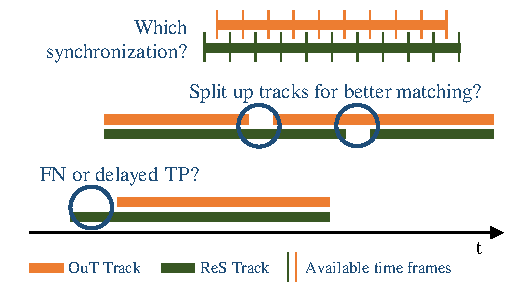
\includegraphics[width=0.49\textwidth]{img/timeline.pdf}
	\caption{Temporal design aspects of a test oracle for TPs, FPs, and FNs.
	}
	\label{fig:timeline}
\end{figure}

%\subsubsection{Temporal validity of tested objects}
%\label{sec:temp_level_of_objects}


\subsubsection{Synchronization of measurement time stamps}
\label{sec:temp_sync}

If the recorded ReS sampling times do not coincide with the OuT sampling times, synchronization of both systems must happen offline during post-processing. % to allow a subsequent comparison.
Continuously present reference tracks from, for example, RTK-GNSS recordings, can be linearly interpolated onto the OuT time stamps \cite[Sec. 10.2.7]{Brahmi2020diss}.

However, in general, reference tracks do not span continuously over the entire recording, which means that the synchronization must also deal with track beginnings and ends. % (Fig. \ref{fig:timeline}, a)).  
If the sampling times of track $a_\text{ReS}$ (Fig. \ref{fig:timeline}) are linearly interpolated to those of $a_\text{OuT}$, all sampling times of $a_\text{OuT}$ are covered. 
Then, however, it is up to the test oracle to decide what happens to the overhanging frames of $a_\text{ReS}$ at the beginning and at the end. 
Both could be neglected, but they could also both mark FNs. 
Whether or not the test oracle identifies FNs there might also depend on whether the overhang falls below a temporal matching threshold given in milliseconds.

For synchronous time stamps of the same frequency that only suffer from a slight offset (smaller than a temporal matching threshold), the test oracle might also synchronize by matching the temporally closest time frames with one another without interpolating any recorded data.


\subsubsection{Matching of objects with an extended lifetime}
\label{sec:temp_matching}

Depending on the perception task whose output is being tested (e.g. detection, filtering, tracking), the tested OuT objects may or may not contain IDs to indicate their correspondence over consecutive time frames. 
In this regard, we assume here that the ReS objects do contain track IDs. 
Resulting OuT object representations that can be matched to the ReS objects are therefore:
\begin{itemize}
\item \textit{detections or ID-stripped single frames out of tracks} (boils down to testing individual decoupled time frames, as explained in Sec. \ref{sec:oracle_simple}, and applied in e.g. the original OSPA metric \cite{schuhmacher2008consistent}) % (if track labels do not matter, e.g. in the OSPA metric \cite{schuhmacher2008consistent})
\item \textit{tracks} (entire OuT and ReS tracks are matched with each other without being split up)
\item \textit{sub-sequences of tracks} (tracks are split up into better-matching sub-sequences, as done in e.g. the CLEAR MOT metrics \cite{bernardin2008evaluating})
\end{itemize}

If only individual frames of tracks are matched irrespective of their belonging to a track, then example b) (Fig.~\ref{fig:timeline}) would contain exactly one FN and one FP. 
If entire tracks are matched, then $b_{\text{OuT},1}$ would match with $b_{\text{ReS},1}$ and $b_{\text{OuT},2}$ would match with $b_{\text{ReS},2}$.
These matches would, however, have large temporal overhangs.
%This would, however, mean that the middle part would stay unmatched despite its geometrical fit. 
To reduce the extent of these overhangs, one could match also sub-sequences of tracks, such as the latest three frames of $b_{\text{ReS},1}$ with the first three frames of $b_{\text{OuT},2}$.
In these cases, some test methods identify an ID switch for $b_{\text{ReS},1}$ to penalize the OuT's fragmented tracking.
% There would still remain two temporal overhangs

\subsubsection{Missed frames and incomplete tracks}
\label{sec:temp_incomplete}

Track $b_{\text{ReS},1}$ (Fig.~\ref{fig:timeline}) is perceived by the OuT in all but one frame, namely the frame in between $b_{\text{OuT},1}$ and $b_{\text{OuT},2}$. 
The test oracle could naturally identify a FN in this missing frame. 
However, if the sampling frequency is sufficiently high such that a single missed frame in the middle is irrelevant to the driving task, the test oracle might also intentionally not want to identify this missed frame as a FN. 

%Contrary to single missed frames in the middle of a ReS track, subsequently missed frames, or missed frames at the end of a track, might be more severe and therefore worth while being identified as FNs.


\subsubsection{Treatment of latency and delays}
\label{sec:temp_latency}

%Similar to missed frames in the middle of a reference track, 
A test oracle should also have a policy for missed frames at the beginning and overhanging frames at the end of a ReS track. 
In example c) (Fig.~\ref{fig:timeline}), the oracle could
\begin{itemize}
	\item identify a FN in the first, missing frame, and TPs otherwise, or
	\item identify just one single TP track, but mark it as detected with an initial delay.
\end{itemize}

Hence, the time that the OuT takes to output a newly appeared object can be considered by the test method implicitly through initial FNs, or explicitly as a property of TPs.
The same concept holds for FPs in case of sustained OuT tracks after the lifetime of a ReS track.



\subsection{Generalization to probabilistic object representations}
\label{sec:oracle_probabilistic}

While the previous two sections assumed deterministic object representations, the following subsections highlight the test oracle's degrees of freedom for evaluating probabilistic data.

\subsubsection{Probabilistic FoVs}
\label{sec:prob_fov}

The FoVs of active sensors often have no clear-cut borders, but their performance can be regarded as degrading probabilistically with increasing distance. 
If a sensor system software does not cut off object hypotheses after a fixed distance, but instead detects objects as far as possible, then a clear distinction of intersecting and overhanging FoV areas of OuT and ReS (Sec. \ref{sec:fov_ref}) is no longer possible.
In such a case, it could be the test oracle that cuts off uncertain FoV regions to reduce the problem to the previously explained deterministic case.
Otherwise, undesired FPs and FNs are possible in these distant regions where one system might randomly still detect an object that the other system might not detect (even though both systems might work perfectly closer to the sensor).


\subsubsection{Probabilistic object distance functions}
\label{sec:prob_bbox}
OuTs often estimate error covariances of the detected objects' positions, orientations, dimensions, and velocities. 
Also the ReS objects' properties are generally uncertain unless they stem from a simulated ground truth \cite{Wang2020inferring_iros}.
It is worth while evaluating the accuracy of these covariances due to their relevance for the downstream driving policy, which could, for example, maintain a higher safety distance to uncertainly perceived objects.

Therefore, finding TP matches requires a probabilistic distance function with a suitable threshold. 
The dissimilarity of two probability distributions for the bounding box centroids can be expressed by the Wasserstein or earth mover's distance.
A probabilistic version of the \textit{IoU} for rotated 3D bounding boxes is the \textit{JIoU} \cite{Wang2020inferring_iros}.

\subsubsection{Probabilistic object existence and classification}
\label{sec:prob_thresholding}

OuTs often compute a confidence for the existence of an object and confidences for its belonging to the different road user classes.
If the OuT does the thresholding itself and only outputs a binary existence and a unique classification, then the deterministic test oracle criteria from Sec. \ref{sec:oracle_simple} can be applied. 
However, if the OuT forwards these probabilities to the downstream driving policy, which could make use of them, then the test oracle should also consider them. 

In the simplest case, the test oracle can threshold the existence confidence at a fixed value and take the class with the maximum classification confidence.
Other oracles might also be reasonable.
For example, if the test oracle refuses to deterministically match OuT bicycles with ReS cars, it might still allow such a match on probabilistic data if the OuT's second most likely classification matches, e.g. $p_\text{OuT,bicycle} = 0.96$ is incorrect, but $p_\text{OuT,car} = 0.95$ is correct for a ReS car.

Furthermore, an oracle's policy for identifying or not identifying FNs behind occlusions could mean that its existence confidence threshold, above which it assumes OuT objects as present, is lower the more the object is occluded.

% \subsubsection{Probabilistic multi-object matching}
% \label{sec:prob_matching}
% THIS IS A BIT EXPERIMENTAL AND I MIGHT DELETE IT LATER
% No binary matches, but rather match probabilities. 
% Just as done with association in probabilistic filters for object tracking (e.g. LMB). 
% I know too little about that to write about it! Leave it out for now!



\section{Exemplary test oracles}
\label{sec:case_studies}

% Or outsource them to the next paper? No, then it would be too theoretical!
% Use as much mathematical notation as possible here! Really? -> Actually, no, this paper will not contain mathematical notation!

The criteria from the previous section (Sec.~\ref{sec:criteria}) are illustrated by two exemplary test oracles in Table~\ref{table:case_study}, namely the evaluation of the nuScenes perception challenge \cite{caesar2019nuscenes} and our own previous test activity \cite{Krajewski2020UsingDrones}. 


Both oracles can be characterized fairly well by the proposed criteria despite their different purposes (ranking of submissions in a leaderboard vs. perception error modeling) and their different reference systems (human labeling on ego vehicle sensor data vs. automated extraction from a hovering drone).


However, even the level of detail of Table~\ref{table:case_study} still does not comprise all relevant information and leaves open uncertainties, especially in terms of ReS data processing and labeling (Sec.~\ref{sec:ref_processing}).


% Mention that these descriptions are still super high-level, and more detail is given (and should be given) in the respective papers and documentation.


% \footnote{\url{https://www.nuscenes.org/tracking}}
% \cite{Krajewski2020UsingDrones}


% WAYMO 3D TRACKING CHALLENGE
% --> don't take it. Was not so popular and is already outdated and even officially retired.
% Describe an example submission at the leaderboard of Waymo Open Dataset. 
% Labeling specifications\footnote{\url{https://github.com/waymo-research/waymo-open-dataset/blob/master/docs/labeling_specifications.md}}.
% Description of perception challenge\footnote{\url{https://waymo.com/open/data/perception/}}

% OLD IDEAS FOR OWN TESTING ACTIVITY
%Use inD data with a simulated ego vehicle and simulated data under test.
%Use the Lanelet2 map (converted to the omega format) to include and exclude certain areas.


% CONTEXT
\newcommand{\scenariosDrone}{Ego vehicle statically observes an urban intersection from a sidewalk.}
\newcommand{\outDrone}{Single lidar sensor with integrated object detection and tracking}
\newcommand{\furtherDrone}{Modeling of how OuT deviates from ReS regarding TP object states}

\newcommand{\scenariosChallenge}{Ego vehicle dynamically participates in various urban traffic scenarios.}
\newcommand{\furtherChallenge}{Computation of metrics such as AMOTA and AMOTP \cite{weng2019baseline} for the online leaderboard}
\newcommand{\outChallenge}{Submitted detection and tracking algorithms that operate on either camera-only, lidar-only, or all raw sensor data}




% DRONE TEST ORACLE
\newcommand{\basicDroneFoV}{ReS FoV is rectangular (about \SI{85}{\meter} $\times$ \SI{45}{\meter}), whereas OuT FoV is \SI{145}{\degree} wide and $\approx$\,\SI{80}{\meter} long. 
The FoVs overlap in the analyzed area.}
\newcommand{\basicDroneOcclusion}{\textit{Not published:} all time steps in which an OuT object was at least marginally occluded to the OuT were removed from its track. % Was the occlusion identified on the OuT object list or on the ReS object list?
}
\newcommand{\basicDroneReSHW}{Camera-equipped drone with 4K resolution hovering in a steady state disturbed by wind.}
\newcommand{\basicDroneReSLabling}{Same as in inD dataset; high-level description of entirely offline post-processing: correcting lens distortion, stabilizing wind disturbances, semantic segmentation by UNet, vehicle localization, then tracking and smoothing by Kalman Filter.}
\newcommand{\basicDroneAreas}{Analyzed area: roads up to non-specified distances from the intersection center. Roads beyond, sidewalks, and anything else is excluded.}
\newcommand{\basicDroneGeometrAlign}{Polynomial transformation of 3\textsuperscript{rd} order from ReS coordinates to OuT coordinates. Polynomial is fitted through corresponding pixels in an orthophoto and a stabilized drone image. 
Accuracy loss in the order of magnitude of $\approx$\,\SI{0.1}{\meter} is not further calculated.}
\newcommand{\basicDroneObjDistance}{2D center distance on the ground plane (threshold below); only car-car matching.}
\newcommand{\basicDroneMultiObjMatching}{Entire tracks are matched (see below). \textit{Not published:} Multiple OuT tracks can be matched to one ReS track (also at the same time), but only one ReS track can be matched to an OuT track (1-to-n).}

\newcommand{\tempDroneSync}{Asynchronous OuT and ReS at \SI{25}{\hertz}; synchronization in post-processing through a mutually captured visual signal; resulting accuracy loss $\approx$\,\SI{0.14}{\meter}. \textit{Not published:} Once synchronized, OuT tracks were interpolated to the matched ReS time stamps, which left overhanging ReS measurements unused.}
\newcommand{\tempDroneMatching}{Entire tracks are matched if their mean center distance (see above) during their non-occluded lifetimes $<$\,\SI{1.5}{\meter}.}
\newcommand{\tempDroneIncomplete}{\textit{Not published:} Two or more incomplete OuT tracks could be matched with one ReS track (see above)}
\newcommand{\tempDroneDelays}{Temporally overhanging track parts are discarded by counting them as FNs or FPs. \textit{Not published:} The closest overhanging OuT measurement was still used for the interpolation onto the ReS time stamp.}

\newcommand{\probDroneFoV}{OuT FoV is acknowledged to have a fuzzy range, but its fuzziness is not explicitly modeled.}
\newcommand{\probDroneObjDistance}{Deterministic distance function only}
\newcommand{\probDroneExistClass}{\textit{Not published:} Objects of any existence confidence were considered without any threshold. Only those parts of OuT tracks during which \textit{car} was the most likely classification were extracted and considered for matching.}


% NUSCENES CHALLENGE TEST ORACLE
\newcommand{\basicChallengeFoV}{ReS FoV $\supseteq$ OuT FoV, both from ego perspective. Ranges are partially defined, but the oracle cuts off ReS and OuT objects beyond class-specific distances.}
\newcommand{\basicChallengeOcclusion}{Implicitly defined by sensor mounting positions and labeling policy. ReS can hardly see behind occlusions of OuT except for a slightly higher mounting position of ReS lidar w.r.t. a camera-only OuT.}
\newcommand{\basicChallengeReSHW}{ReS HW (cameras, lidar, radar, GNSS+IMU) $\supseteq$ OuT HW}
\newcommand{\basicChallengeReSLabling}{See human annotator instructions\tnote{b}. They are clear and detailed, but cannot rule out all uncertainties (when ``reasonably sure" about object shape and location, use ``best judgment" on bounding box properties). ReS objects must have at least 1 lidar or radar point. ``Multiple validation steps" \cite{caesar2019nuscenes}. %, which might lead to confusion in specific cases\tnote{c}.
}
\newcommand{\basicChallengeAreas}{No evaluation beyond class-specific maximum detection and tracking ranges (\SI{40}{\meter} to \SI{50}{\meter}); no evaluation of bikes and motorcycles inside bike racks; list of excluded object classes.}
\newcommand{\basicChallengeGeometrAlign}{Verbally documented calibration of lidar, camera, and radar w.r.t. ego coordinate system; without accuracy estimate. ReS-OuT-alignment might be imperfect for the camera-only OuT.}
\newcommand{\basicChallengeObjDistance}{2D center distance on the ground plane; threshold of \SI{2}{\meter}; a match requires equal object classifications.}
\newcommand{\basicChallengeMultiObjMatching}{Metrics from \cite{Bernardin2006mot_metrics} use 1-to-1 matching and Munkres' algorithm (see \cite{bernardin2008evaluating}).}

\newcommand{\tempChallengeSync}{Online synchronization of lidar (\SI{20}{\hertz}) and camera (\SI{12}{\hertz}), but evaluation only on keyframes (\SI{2}{\hertz}) where the sensors coincide. Radar operates on \SI{13}{\hertz}. ReS tracks and OuT tracks are linearly interpolated ``to avoid excessive track fragmentation from lidar/radar point filtering".}
\newcommand{\tempChallengeMatching}{Metrics from \cite{Bernardin2006mot_metrics} keep a match over subsequent time steps for as long as it is below the threshold, even if another, new match candidate would have even less cost.}
\newcommand{\tempChallengeIncomplete}{All missed frames are counted as FNs; additionally, the LGD (average longest gap duration in seconds) is computed.}
\newcommand{\tempChallengeDelays}{Temporally overhanging track parts are counted as FNs or FPs; additionally, the TID (average track initialization duration in seconds) is computed.}

\newcommand{\probChallengeFoV}{FoVs are not modeled probabilistically}
\newcommand{\probChallengeObjDistance}{Deterministic distance function only}
\newcommand{\probChallengeExistClass}{The oracle expects an existence confidence $\in [0,1]$ in each time step, and a temporally constant classification $\in \{\textrm{car}, \textrm{pedestrian}, \dots\}$.  Metrics in further evaluation \cite{weng2019baseline} average per class over 40 different recall values, which stem from a varied existence confidence threshold of the oracle. } % Note: the existence confidence of a TP object is called "score" in https://github.com/xinshuoweng/AB3DMOT/blob/master/scripts/KITTI/evaluate.py#L365





\begin{table*}[htbp]
	\begin{threeparttable}
	\centering
	\caption{Different test oracles for TP, FP, FN, expressed in the terminology of this paper}
	\label{table:case_study}
	\begin{tabularx}{\linewidth}{
			>{\hsize=0.02\hsize}X
			>{\hsize=0.38\hsize}X 
			>{\hsize=0.8\hsize}X 
			>{\hsize=0.8\hsize}X 
		}
		\toprule
		\multicolumn{2}{>{\hsize=\dimexpr0.4\hsize+0.4\tabcolsep+\arrayrulewidth\relax}X}{\textbf{Criterion}}                                         & \textbf{Evaluation of nuScenes tracking challenge\tnote{a}} & \textbf{Obtaining TPs for perception error modeling \cite{Krajewski2020UsingDrones}} \\ \midrule
		\parbox[t]{2mm}{\multirow{3}{*}[-0.4cm]{\rotatebox[origin=c]{90}{(\textit{Context})}}} & Scenarios                                           & \scenariosChallenge                  & \scenariosDrone                                                                 \\ \cline{2-4}
																								& OuT                                                 & \outChallenge                        & \outDrone                                                                       \\ \cline{2-4}
		                                                                                        & Further evaluation after TP, FP, FN                 & \furtherChallenge                    & \furtherDrone                                                                   \\ \midrule
		\parbox[t]{2mm}{\multirow{8}{*}[-2.5cm]{\rotatebox[origin=c]{90}{Basic}}}               & \ref{sec:fov_ref} FoVs                              & \basicChallengeFoV                   & \basicDroneFoV                                                                  \\ \cline{2-4}
		                                                                                        & \ref{sec:occlusions} Occlusion handling             & \basicChallengeOcclusion             & \basicDroneOcclusion                                                            \\ \cline{2-4}
		                                                                                        & \ref{sec:ref_hw} ReS hardware                       & \basicChallengeReSHW                 & \basicDroneReSHW                                                                \\ \cline{2-4}
		                                                                                        & \ref{sec:ref_processing} ReS labeling               & \basicChallengeReSLabling            & \basicDroneReSLabling                                                           \\ \cline{2-4}
		                                                                                        & \ref{sec:semantic_areas} No-test areas             & \basicChallengeAreas                 & \basicDroneAreas                                                                \\ \cline{2-4}
		                                                                                        & \ref{sec:geometrical_alignment} Geometr. alignment  & \basicChallengeGeometrAlign          & \basicDroneGeometrAlign                                                         \\ \cline{2-4}
		                                                                                        & \ref{sec:distance_function} Obj. distance func.     & \basicChallengeObjDistance           & \basicDroneObjDistance                                                          \\ \cline{2-4}
		                                                                                        & \ref{sec:multi_object_matching} Multi-obj. matching & \basicChallengeMultiObjMatching      & \basicDroneMultiObjMatching                                                     \\ \midrule
		\parbox[t]{2mm}{\multirow{4}{*}[-1.2cm]{\rotatebox[origin=c]{90}{Temporal}}}            & \ref{sec:temp_sync} Synchronization                 & \tempChallengeSync                   & \tempDroneSync                                                                  \\ \cline{2-4}
		                                                                                        & \ref{sec:temp_matching} Matching                    & \tempChallengeMatching               & \tempDroneMatching                                                              \\ \cline{2-4}
		                                                                                        & \ref{sec:temp_incomplete} Incomplete tracks         & \tempChallengeIncomplete             & \tempDroneIncomplete                                                            \\ \cline{2-4}
		                                                                                        & \ref{sec:temp_latency} Delays \& latency            & \tempChallengeDelays                 & \tempDroneDelays                                                                \\ \midrule
		\parbox[t]{2mm}{\multirow{3}{*}[-0.2cm]{\rotatebox[origin=c]{90}{Probabilistic}}}       & \ref{sec:prob_fov} FoVs                             & \probChallengeFoV                    & \probDroneFoV                                                                   \\ \cline{2-4}
		                                                                                        & \ref{sec:prob_bbox} Obj. distance func.             & \probChallengeObjDistance            & \probDroneObjDistance                                                           \\ \cline{2-4}
		                                                                                        & \ref{sec:prob_thresholding} Obj. exist. \& class.   & \probChallengeExistClass             & \probDroneExistClass                                                            \\ \bottomrule
	\end{tabularx}
	\begin{tablenotes}
		\item [a] \href{https://www.nuscenes.org/tracking}{https://www.nuscenes.org/tracking}
		\item [b] \href{https://github.com/nutonomy/nuscenes-devkit/blob/master/docs/instructions_nuscenes.md}{https://github.com/nutonomy/nuscenes-devkit/blob/master/docs/instructions\_nuscenes.md}
	%	\item [c] \href{https://github.com/nutonomy/nuscenes-devkit/issues/366}{https://github.com/nutonomy/nuscenes-devkit/issues/366}
	\end{tablenotes}
	\end{threeparttable}
\end{table*}
% \multicolumn{2}{>{\hsize=0.5\hsize}X}{\textbf{Criterion}}
% \multicolumn{2}{|>{\hsize=\dimexpr0.5\hsize+0.5\tabcolsep+\arrayrulewidth\relax}X|}{\textbf{Criterion}}
% \parbox[t]{2mm}{\multirow{1}{*}{\rotatebox[origin=c]{90}{aaa}}}

%\subsection{How do TP statistics change when the oracle criteria vary?}
%I could include such a case study on simulated data. The omega format with the perception testing dashboard would be handy for that.
% It is good for illustration purposes, but shows nothing special because it is only expected that the statistics change. 
% Though, it could serve as a demonstration of *how much* statistics change. 


\section{Discussion of Research Questions}
\label{sec:discussion}

% TODO: organize this discussion logically: w.r.t. research questions, but also w.r.t. what else I found out. 

This section discusses the three research questions introduced in the Introduction (Sec. \ref{sec:introduction_contrib}). 


\subsection{RQ1: Can TP, FP, and FN be objectively defined?}
\label{sec:discussion_rq1}

No, due to ambiguity in ReS labeling (Sec. \ref{sec:ref_processing}), which needs either human work or neural networks, both of which is impossible to fully specify. 

But it can be defined as objectively as possible or feasible, and this paper is a major step in this direction. 

\subsection{RQ2: How relevant are TP, FP, and FN for task-oriented perception metrics?}
\label{sec:discussion_rq2}



\subsection{RQ3: Can statistics of TP, FP, and FN contribute to a safety argumentation?}
\label{sec:discussion_rq3}

TODO mention that even our own test oracle was originally not fully described in the original publication. We had to look up source code for certain information in Table~\ref{table:case_study}.



\subsection{REST OF STUFF THAT I WANT TO INCLUDE IN THE DISCUSSION (UNORGANIZED)}

We have presented a generic set of relevant conditions for specifying a test oracle that identifies TP, FP, and FN. 
However, even this set of conditions might not be generic enough to specify all possible concepts of such a test oracle. 


\subsubsection{Awareness of Symbol Grounding Problem}

TODO

Just like it is hard to define what e.g. a pedestrian is, it is also hard to define what a true positive is. 
Humans that use these terms in their natural language have learned their meanings over time, but are often not fully aware of the exact criteria that define a pedestrian or a true positive, for example.  

Humans tend to say ``the ADS did not see the pedestrian". While for some world model instances, such a statement is obvious, for other world model instances, it is highly complex to unambiguously define what it means that one road user sees another one. 


\subsubsection{Design of Future Safety-Oriented Perception Metrics}

Metrics that rely on a distinction between, TPs, FPs, FNs have these difficulties. 

In contrast, Task-Oriented Metrics that employ a downstream driving function or assumptions thereof don't manually feature-engineer the criteria for must-see objects, but have that additional complexity. 


\subsection{Compliance with standards}

TODO

Some standards, e.g. UL4600 \cite[Sec. 8.4.1.2]{UL4600_voting_2019} suggest providing statistics of FPs and FNs. 
Since a safety argumentation to comply with a standard should contain the least possible ambiguity, this paper aims at providing guidance to define FPs and FNs as clearly as possible. 



\subsection{More formal definition of test oracle}

It is hard because some things are hard to formalize.
A modular technical description of a test oracle would already partially predetermine the arrangement of its modules, or the internal structure of the test oracle. This, however, can be flexible. For example, certain objects or semantic areas could be ignored at the very beginning of the testing activity, or at the very end. 
Future work how far a formal description can go without unnecessarily prescribing internals of the test oracle. 



\section{Related Work}
\label{sec:related_work}

Only related work here that is about the definition of TPs, FPs, and FNs. 
All further relevant literature sources that do not explicitly focus on defining TPs will be referenced as they become relevant in other sections. 

Florbäck et al. \cite{Florbaeck2016.matching.offline} and Sondell and Svensson \cite{Sondell2018} investigate how machine learning can reproduce human associations of objects under test to reference objects.


\section{Conclusion}
\label{sec:conclusion}

Future work includes a more formal description of a test oracle, potentially by means of mathematical notation or a domain-specific language.

\section*{Acknowledgment}
\label{sec:acknowledgment}

Open Access funding enabled and organized by Projekt DEAL. % of RWTH Aachen University Library.
Besides this, the present work was conducted independently without related \href{https://ko-fi.com/michaelhoss}{funding} or employment. 
% The author would like to thank the social media commenters for their feedback on the given topic.

%\section{Introduction}
\label{sec:introduction}

Will refer to \cite{Hoss2022review}.

% \section{Related Work}
\label{sec:related_work}

% \section{Method}
\label{sec:method}

Describe your experimental design with enough detail so that a competent colleague could reproduce your results. Passive voice sometimes functions well in the Methods section.
Elsewhere in a scientific paper, however, it should rarely be chosen. 

\begin{figure}
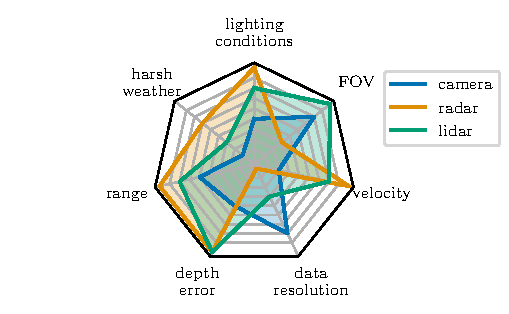
\includegraphics{img/spider_sensorcomp.pdf}
\centering
\caption{Figures MUST be in PDF (everything that can be a vector must be a vector) or PNG format to prevent issues with the arXiv upload.}
\label{fig:compare_sensors}
\end{figure}

% \section{Evaluation}
\label{sec:evaluation}


% \section{Conclusion}
\label{sec:conclusion}

Discussion and Outlook
% \section{Acknowledgment}
\label{sec:acknowledgment}

This work results partly from the KIGLIS project supported by the German Federal Ministry of Education and Research (BMBF), grant number 16KIS1231.

% -------------------------- REFERENCES -------------------------------

{\small
\bibliographystyle{IEEEtran}
\bibliography{literature/AllSourcesMHO.bib}
}

\end{document}
